\documentclass[preprint,10pt,5p,twocolumn]{elsarticle}
%\documentclass[preprint,authoryear,10pt,5p,twocolumn]{elsarticle}

\usepackage{amsmath}
\usepackage{graphicx}
\usepackage{subfigure}
\usepackage{array}
\setlength{\extrarowheight}{0.3cm}

%% for the old format  ( remove this and the abstract and the bibgraphy style. )
%\documentclass{article}
%\usepackage{spconf}
%\usepackage{amsmath}
%\usepackage[dvips,pdftex]{graphicx}
%\usepackage{named}
%\usepackage[dvips,pdftex]{hyperref}

%\title{Sketch Recognition using Particle Swarm Optimizations}
%\twoauthors
%  {Maha El Meseery\sthanks{Corresponding Author}, Mahmoud Fakhr El Din\sthanks{Associate Professor}, Samia Mashali\sthanks{Professor}}
%	{Signals Processing Group \\ Computers and Systems Department \\
%  Electronic Research Institute\\Cairo, Egypt\\
%	melmeseery@eri.sci.eg, mafakhr@mcit.gov.eg,\\ samia@eri.sci.eg}
%  {Magda Fayek\sthanks{Associate Professor}, Nevin Darwish\sthanks{Professor}}
%	{Computer Engineering Department\\
%	Faculty of Engineering \\Cairo University\\Cairo, Egypt\\
%	magdafayek@gmail.com,ndarwish@ieee.org}
%\maketitle

\begin{document}
\begin{frontmatter}
\title{Sketch Recognition using Particle Swarm Optimizations}

%% use optional labels to link authors explicitly to addresses:
%% \author[label1,label2]{<author name>}
%% \address[label1]{<address>}
%% \address[label2]{<address>}

\author[ERI]{Maha El Meseery\footnote{Corresponding author}}
\author[ERI]{Mahmoud Fakhr El Din}
\author[ERI]{Samia Mashali}
\author[FAC]{Magda Fayek}
\author[FAC]{Nevin Darwish}
\address[ERI]{Signals Processing Group, Computers and Systems Department, 
  Electronic Research Institute, Cairo, Egypt\\melmeseery@eri.sci.eg, mafakhr@mcit.gov.eg, samia@eri.sci.eg}
\address[FAC]{Computer Engineering Department,
	Faculty of Engineering, Cairo University, Cairo, Egypt\\
	magdafayek@gmail.com, ndarwish@ieee.org}
\begin{abstract}
%%This study 
Sketches and drawings are widely used as simple methods of expressing thought and designs. The goal of this paper is developing a sketch recognition system that facilitates using sketches in computer systems. The system uses the Particle Swarm Optimization (PSO) algorithm to optimally segment the strokes the user draws into meaningful geometric primitives.  These geometric primitives are grouped to form symbols which are further identified using a Support Vector Machines (SVM) classifier. Two versions of PSO segmentation algorithms were implemented. Experiments were conducted on three different datasets, simple presentation (Hs-DS), Electrical Design (EL-DS) and Logic Design (LD-DS) symbols. Results show that both PSO algorithms produce better segmentation than most current systems. This segmentation improvement contributed in getting more accurate recognition results on all the datasets tested. The results prove that the system is effective especially in datasets with low diversity in shapes, i.e., similar shapes, as in Logic Design dataset (LD-DS). %The results prove the effectiveness of the proposed system on various dataset, especially datasets with low shape diversity as in Logic Design dataset (LD-DS).% effectiveness of the proposed system on various dataset, especially datasets with low shape diversity as in Logic Design dataset (LD-DS). %Result show that the system is especially effective on dataset with % sketch are divided Users draw symbols and sketches using a set of pen strokes. 
%%Sketch recognition is defined as the process of identifying symbols that users draw using single or multiple strokes. Usually, users draw strokes using pens. The sketch recognition system immediately interprets their strokes as objects that can be easily manipulated. This paper uses Particle Swarm Optimization (PSO) to divide the strokes the user draws into meaningful geometric primitives. These geometric primitives are grouped to formulate symbols which are further identified. The results show that using PSO improves segmentation results which guide the symbol recognition phase. As for recognition we use Support Vector Machines (SVM) classifier which further improves the final recognition accuracy.  

\end{abstract}

\begin{keyword}
%% keywords here, in the form: keyword \sep keyword
Symbol Recognition, Discrite Particle Swarm Optimization (DPSO), Sketch Recognition, Geometrical Features, Polygon approximation
%% PACS codes here, in the form: \PACS code \sep code

%% MSC codes here, in the form: \MSC code \sep code
%% or \MSC[2008] code \sep code (2000 is the default)

\end{keyword}

\end{frontmatter}



%\begin{abstract}
%%This study 
%Sketches and drawings are widely used as a simple method of expressing thought and designs. The goal of this paper is developing a sketch recognition system that facilitates using sketches in computer systems. The system uses Particle Swarm Optimization (PSO) algorithm to optimally segment the strokes the user draws into meaningful geometric primitives.  These geometric primitives are grouped to formulate symbols which are further identified using a Support Vector Machines (SVM) classifier. Two different segmentation algorithms were evaluated and results show that both algorithms improve the final recognition results. Experiments were conducted on three different dataset, simple presentation (Hs-DS), Electrical Design (EL-DS) and Logic Design (LD-DS) symbols. Results show that the effectiveness of the proposed system on various dataset especially on datasets with low shape diversity as in Logic Design dataset (LD-DS).  % sketch are divided Users draw symbols and sketches using a set of pen strokes. 
%%Sketch recognition is defined as the process of identifying symbols that users draw using single or multiple %strokes. Usually, users draw strokes using pens. The sketch recognition system immediately interprets their %strokes as objects that can be easily manipulated. This paper uses Particle Swarm Optimization (PSO) to divide %the strokes the user draws into meaningful geometric primitives. These geometric primitives are grouped to %formulate symbols which are further identified. The results show that using PSO improves segmentation results %which guide the symbol recognition phase. As for recognition we use Support Vector Machines (SVM) classifier %which further improves the final recognition accuracy.  
%\end{abstract}
\pagenumbering{arabic}
\section{Introduction}

Computer research nowadays aims at facilitating computer human interaction in every way. Pen-based interfaces give the user a pencil-paper like feeling that enhances interaction more than the current used keyboard-mouse computer interfaces. However, using sketches as input to a computer system requires the system to understand the drawn sketches. In a truly freely sketch system this is not a trivial problem due to the sloppy and messy way in which users draw sketches. Sketches here stand for any hand drawing the user draws using digital stylus or similar device. Normally, sketches are composed of a set of strokes. The time between pen-up and pen-down events identifies each stroke. The strokes are mainly the path of points, which the user draws between the pen-down and pen-up events while using the stylus or similar device. 

Sketch recognition can be applied using either Pattern Recognition (PR) based method or Artificial Intelligence (AI) based method. In AI based methods, Symbols are represented using hierarchical levels of simpler geometric shapes or primitives and spatial relations between them. Systems that employ such representation must first pre-process strokes to break them into geometric primitives. Recognition can then is treated as an AI problem which can be solved using methods like sub graph matching, Bayes belief network, and constrain satisfaction. A Hierarchical shape description was widely used in sketch systems \cite{HierarchicalParsing7,SketchRead2007}.  %Ladder30,AlvaradoFreedom42


Recognition based on AI methods as applied in \cite{SketchRead2007} has the principle problem of computational complexity of the matching between shape description and geometric primitives produced in the segmentation process. Natural sketch are difficult to be segmented and grouped to create reliable fragment of geometric primitives. This is partially due to the increase of noise and other phenomena such as overlapped, over traced strokes and sharing of strokes between different symbols. Since these systems are dependable on the segmentation results, they either perform recognition using undependable segmentation results or consider different ways to segment the input sketch. This is because they assume that each stroke plays a role in the structure of the shape. 
 
In PR based methods, systems compute properties that describe symbols then use a classification method to recognize symbols. The properties used can either be based on gesture properties, global shape properties or image based properties. Gesture properties are set of features that represent how the user draws a symbol not how it looks like (e.g., identify a rectangle when a user draws a L corner). In gesture properties approach, systems identify symbols by using gesture properties of some of its underlying strokes. A system that uses gestures properties assumes that users draws symbols in specific order and style \cite{gestureexample12,aideddesgin22}. In global shape properties approach, systems investigate general shape properties and its underlying strokes. Using shape properties (e.g., ratio of the area of convex hull to the area of shape) relaxes the assumption and the role of each stroke in the symbol but it does not truly represent the appearance or fine details of the symbol \cite{DiagramOfflineConvexHull,Cali63}. Unlike shape properties based methods, image based methods disregard individual strokes and focus on the overall appearance of shapes. These system convert the shapes into image and extracted image based features (e.g. local gradient feature)\cite{Oltmans07,imagetrainable48}. In \cite{imagetrainable48}, they used four different distance measures to match user symbol with the prototype database. The prototype of a shape is represented as an image of the symbol that is normalized and scaled.  However, the problem is that the shape prototype must represent all transformation and variation the input shape can have.   %Image based methods are used in \cite{Oltmans07,imagetrainable48} where they computed a code book of 1000 features to recognize symbols. 

Methods based on gesture and global shape properties produce systems that are dependent on assumptions about how strokes can be grouped. These systems assume that users will finish drawing a shape before moving to the next one \cite{Cali63,geometrydomain49}. This assumption allows the system to temporally group strokes and then recognizes them based on their strokes or global shape properties. Alvarado \cite{AlvaradoDigital} argued that this assumption does not hold in natural sketches. 


In this paper, we choose to implement a hybrid method that includes shape property, gesture and hierarchical information. Our method attempts to avoid many of the problems faced by approaches based on individual gestures or global shape properties while trying to gain the additional information that the stroke based system uses. Firstly, the system uses particle swarm optimization (PSO) to optimally segment user's strokes. Users can draw symbols using any number of strokes in any order they like. The system segments each stroke using two different PSO algorithms. The first segmentation algorithm is based on dividing the digital curve into polygons\cite{PolygonApproximationPSO}. Our algorithm enhances its performance by adding curvature and other local information during segmenting strokes to achieve better results. To handle complex strokes, our system uses a second segmentation PSO algorithm that segment strokes into a set of lines and circular arcs. The two segmentation algorithms can either by used  individually or in parallel then chosing the segmentation that gives the minimum error. After segmentation, a feature vector composed of different statistical, geometrical and composite features is deduced. The final classification step uses a SVM classifier to classify symbols into one of the previously trained classes based on the features vector computed.


 The remaining of the paper is as follows; the literature review on stroke segmentation is presented in Section \ref{sec:review}. Section \ref{sec:ParticleSwarmAlgorithm} introduces Particle Swarm Optimization. Section \ref{Sysdisc} describes the proposed system in details. Section \ref{sec:Experiments} describes the results obtained from the experiments that were preformed. Finally, the conclusion and future work is presented in Section \ref{ConclusionandFutureWork}.  

\section{Literature Review}
\label{sec:review}

Yu \cite{meanshift10} introduced a \textit{feature area} for each primitive and then computed the segmentation error for different types of primitives based on the computed \textit{feature area}. His system achieved good accuracy in simple shapes (square, ellipse,...etc) but did not perform well in complex shapes. A hybrid algorithm was introduced in \cite{earlyprocess}\footnote{Alg3 used in Section \ref{sec:Experiments} } where different sets of segments are generated based on both curvature and speed dominant points, followed by choosing a segmentation with the least error from a generated hybrid set. However, this system is limited to recognizing only specific simple geometric shapes with a set of low level recognizers. Each low level recognizer is designed to recognize only one geometric shape using spatial and geometric information extracted from input stroke. 

A genetic algorithm was used by \cite{CruveDivisionSwarm} to optimally divide digital curves into lines and curves. Chen et al. \cite{CruveDivisionSwarm} uses digital curves scanned from paper as input to the system. However, they did not take the advantage of the curvature or local geometric properties of the digital curve. Yin \cite{PolygonApproximationPSO} used PSO to convert digital curves into polygons. Our system adopts Yin \cite{PolygonApproximationPSO} method and tries to improve it by adding curvature and other local information while segmenting strokes to achieve better segmentations. The next section presents the general particle swarm algorithm used in the proposed system.

 % are presented in section \ref{subsubsec:Discreteparticleswarmalgorithm}

\section{Discrete Particle Swarm Optimization}
\label{sec:ParticleSwarmAlgorithm}
 The main idea of \textit{Particle Swarm Algorithm (PSO)} is to represent each solution with a $N$ dimension particle from the solution space \cite{PSOFirst}. Each particle moves with a direction and velocity $v_{ij}$ based on equations \ref{eq:Swarm1} \& \ref{eq:Swarm}.

\begin{equation}
%\[
p_{ij}=p_{ij}+v_{ij},
%\
\label{eq:Swarm1}
\end{equation}
 
where $p_{ij}$ represent the $j$th dimension in the $i$th particle and $v_{ij}$ is the velocity of the $j$th dimension in the $i$th particle.
 %Equation [\ref{eq:Swarm}] shows how velocity and direction of each particle are computed
 \begin{equation}
v_{ij}  = v_{ij} \omega + c_1 r_1 (lbest_{ij}  - p_{ij} ) + c_2 r_2 (gbest_{ij}  - p_{ij} ),
\label{eq:Swarm}
\end{equation}
 where $\omega$ is the inertia weight parameter which controls the tradeoff between exploration and exploitation,  $lbest_{ij}$ is the local best particle, $gbest_{ij}$ is the global best particle, $r_1$ \& $r_2$ are random variables and $c_1$ \& $c_2$ are the swarm acceleration parameters.

 After each iteration the global best $g_{best}$ particle and the agent local best particle $l_{best}$are evaluated based on the maximum fitness functions of all particles in the solution space. The solution is found after achieving a specific number of iteration or after an error threshold is achieved.
Equation \ref{eq:descrite} is used to change the general swarm algorithm into binary particle (\textit{Discrete Particle Swarm Algorithm DPSO}). The \textit{DPSO} handles particle values of either $0$ or $1$ \cite{PSODisceret}.  
\begin{equation}
   P(i)\Leftarrow 
\left \{
\begin{array}{c} 
1 \quad \quad if\quad r_{3}>p_{i}  \\

0 \quad \quad if\quad r_{3}<p_{i}, 
\label{eq:descrite}
\end{array}\right.
\end{equation}
 where $p_{ij}$ is the numerical values of the particle and $r_{3}$ is a random variable. 


\section{The Proposed System}
\label{Sysdisc}
 The suggested sketch recognition system is divided into three main steps; 1) preprocessing, 2) segmentation and 3) Recognition. The following section provides a detailed description of each step.
 
\subsection{Preprocessing}
\label{Prepross} 
 Speed and time difference information were widely used in sketch recognition systems \cite{earlyprocess}. Figure \ref{fig:orignalStroke} shows an example of an input stroke drawn by users.  Figure \ref{fig:speed2Distance} shows the graph of time difference and the speed for the stroke in Figure \ref{fig:orignalStroke}. It was noted that time difference provides more distinct maxima than the speed information. Agar et al. \cite{polygonfeedback31} mentions that the pointing device (e.g., mouse) sampling rate is the reason for this phenomenon. The points are sampled at regular time intervals as long as the pointing device is moving. Therefore, there are no new detected points when the pointing device is stationary. This leads to a nearly constant time difference between samples while the pen is moving and large difference while the pen is stationary (Figure \ref{fig:timediff}). Contrary to time difference information, the speed information has a lot of noise in the data because usually  users draw with variant speeds (Figure \ref{fig:speed2Distance}).  %Similarly, direction information is used as it provides better distinctive maxima for the corners than the curvature information \cite{meanshift10}.% Figure \ref{fig:curvatures} shows the direction and curvature graphs for the stroke drawn in Figure \ref{fig:orignalStroke}

 \begin{figure}[h]
	\centering
		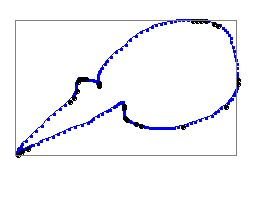
\includegraphics[scale=0.5]{images/stroke3.jpg}
	\caption{Input Stroke} Example of an input stroke to the system. 
	\label{fig:orignalStroke}
\end{figure}

 \begin{figure}
	\centering
			\subfigure[Speed versus Displacement Graph]{	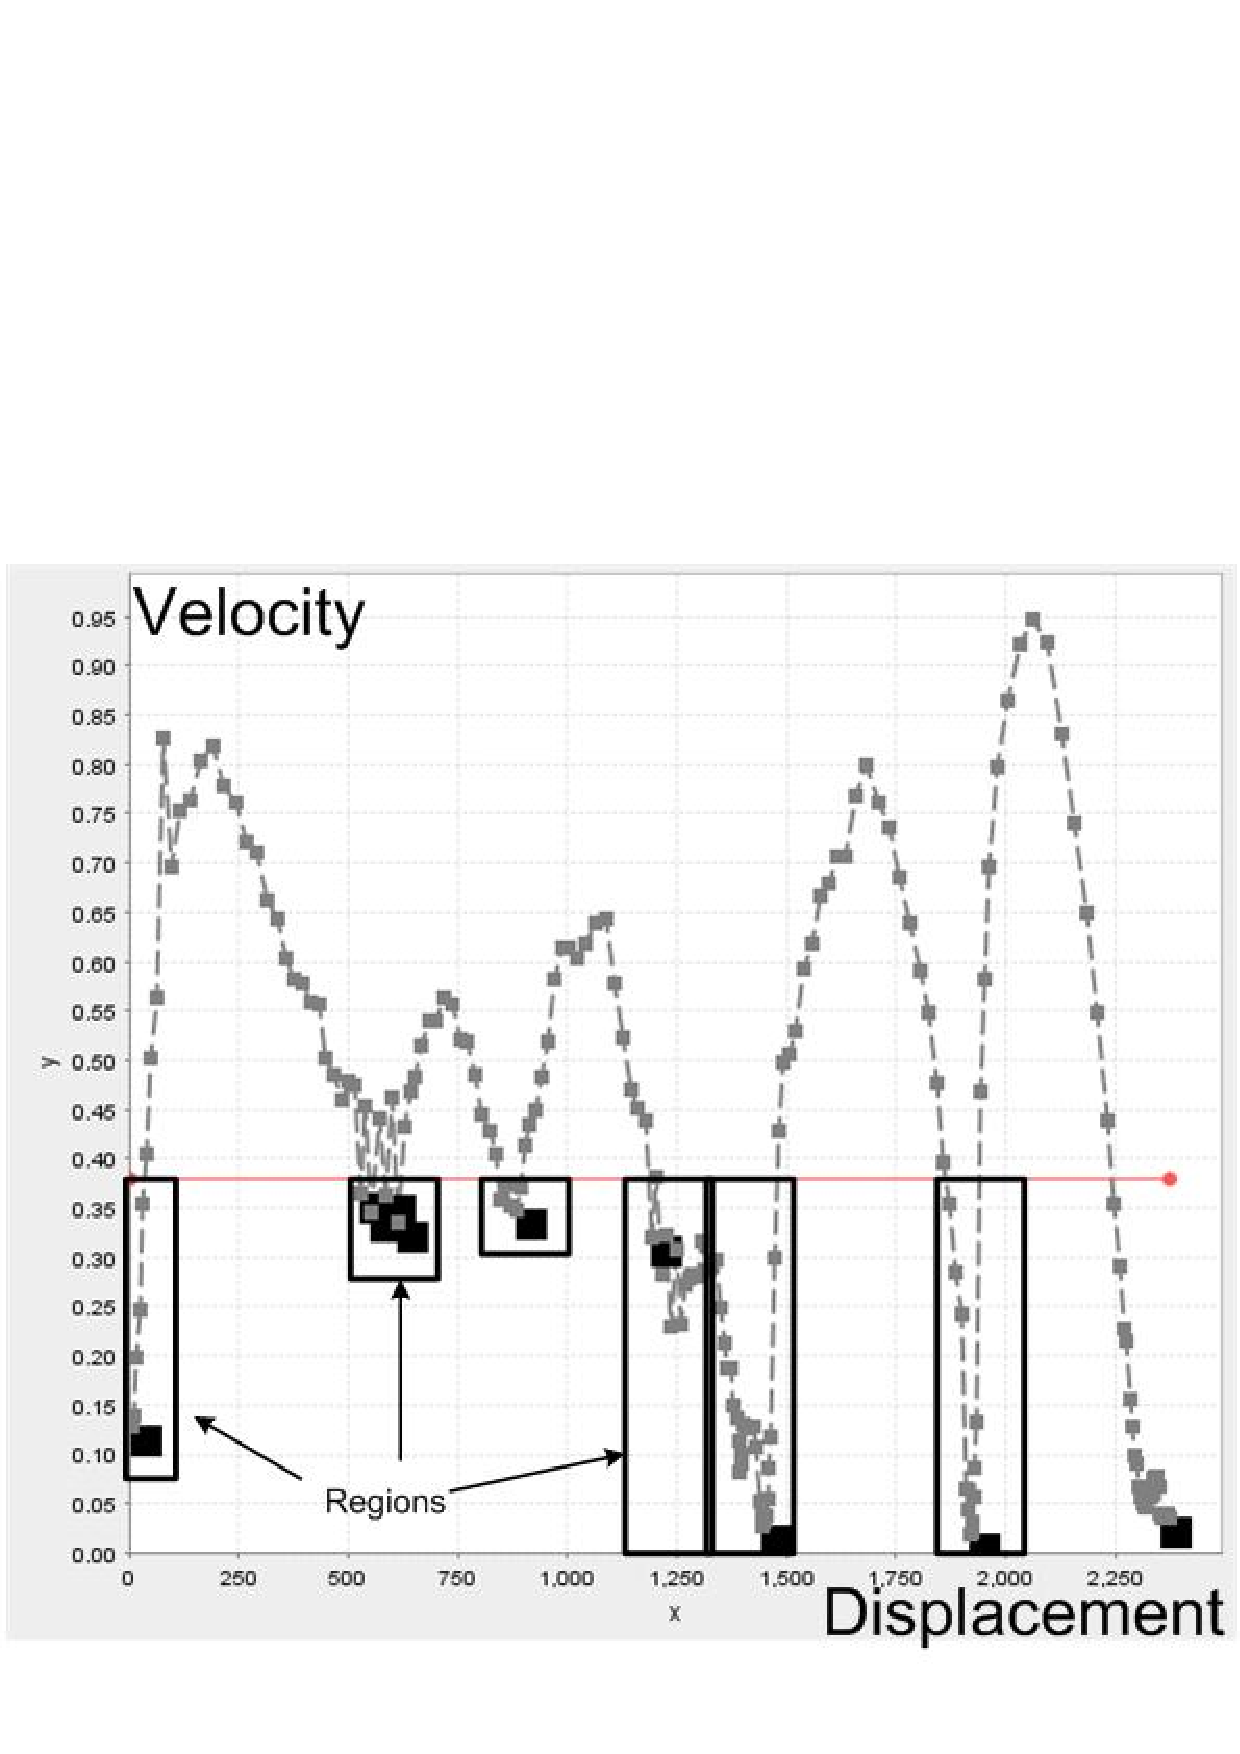
\includegraphics[scale=0.4]{images/vel3.jpg}}
			\hfill
			\subfigure[ Time Difference  versus Displacement Graph] {\label{fig:timediff}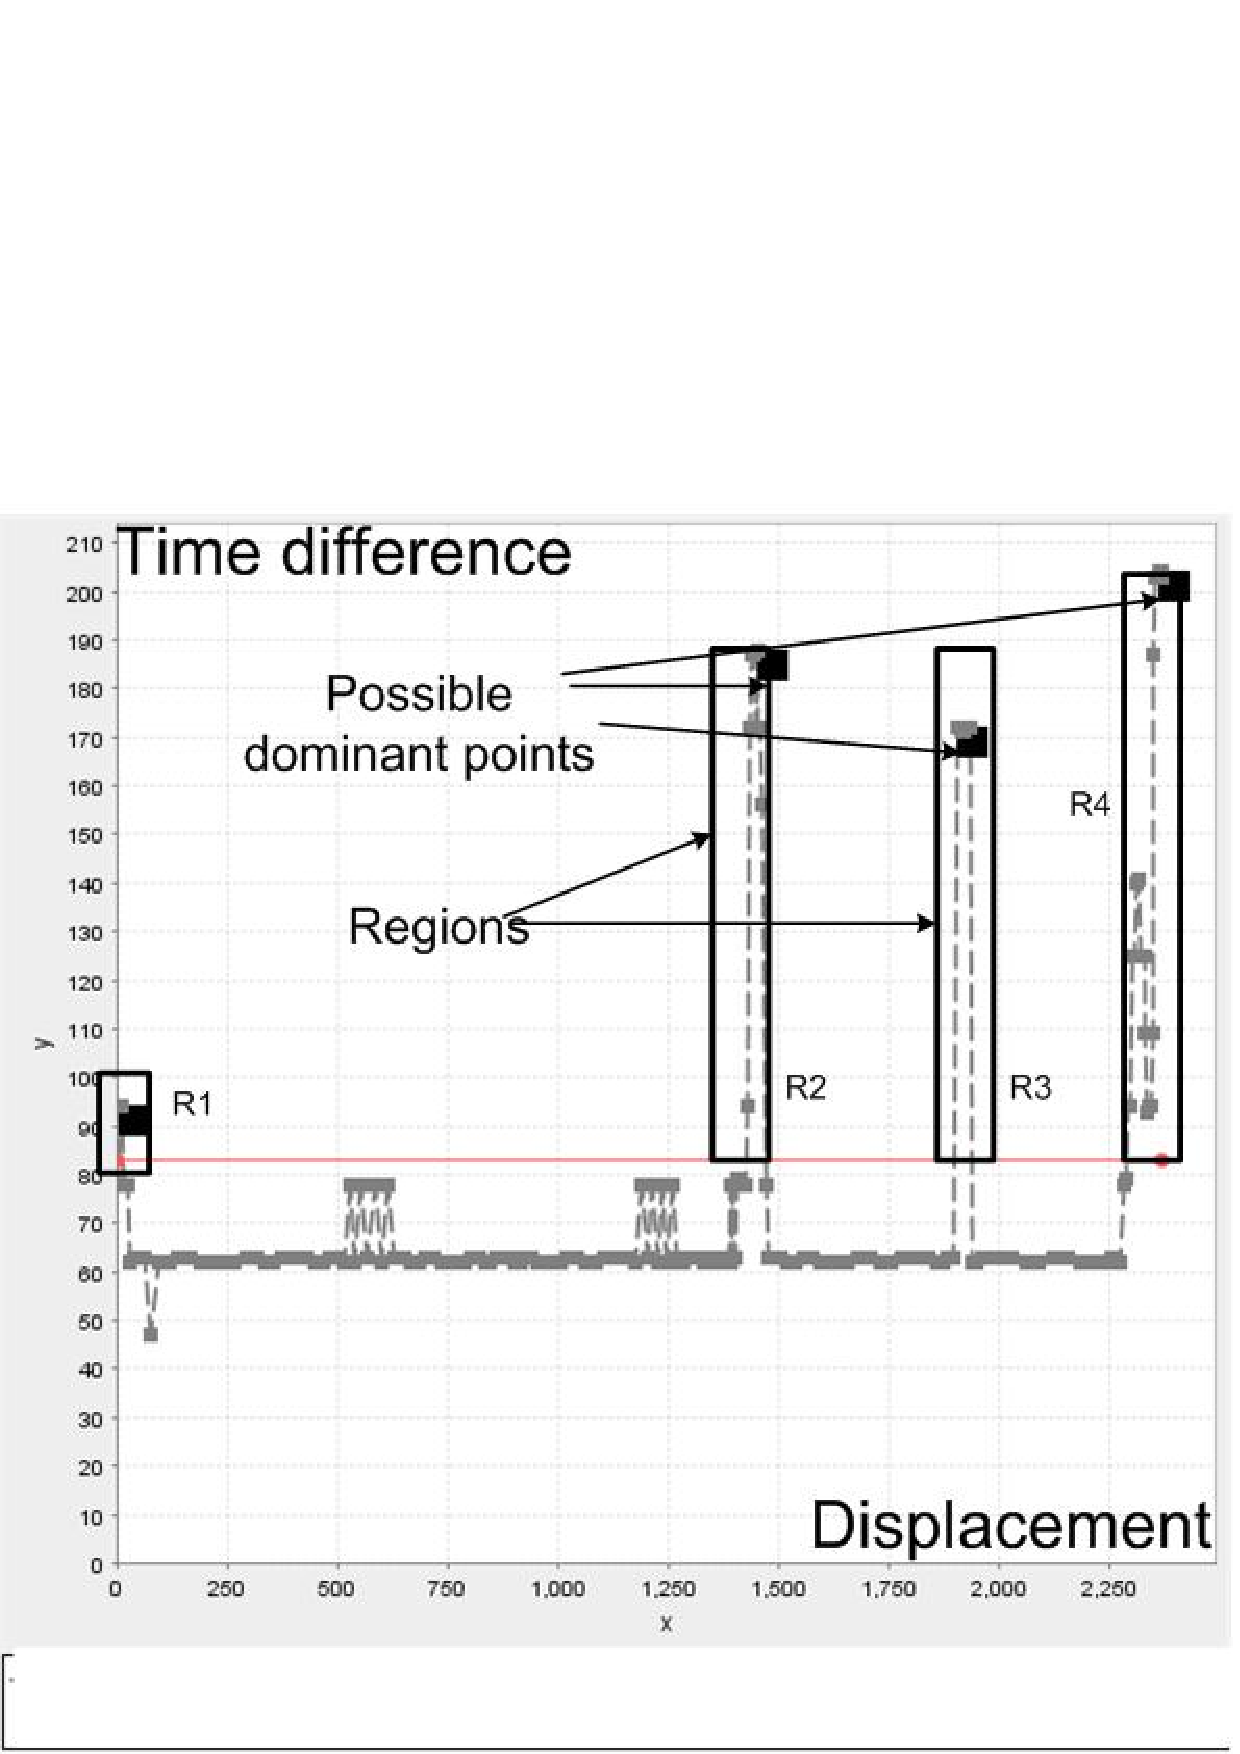
\includegraphics[scale=0.4]{images/td3.jpg}}
	\caption{Speed and Time Difference Graphs}  a) speed graph has lot of noise in the data with respect to b) time difference.   The black points denote the location of the possible dominant points $P_{pd}$. Black rectangles represent regions $R_i$ that in a) Are lower than the threshold. b) Are above the threshold. 
	\label{fig:speed2Distance}
\end{figure}
 
Dominant points are characterized by low speed values, high curvature and direction values. However, the dominant points from the curvature information may not be the same points as the dominant points extracted from the speed information. Hence, we compute time difference, direction, speed and curvature of each point along a stroke to ensure that no dominant point is overlooked in this phase. The speed is calculated as $v=\Delta s/\Delta t$ where $t$ is the time difference between two points and $s$ is the length between them. The direction $d$ calculated as the angle between vectors $\overrightarrow {P_{i - 1} P_i }$ and the $x-axis$ and the curvature is considered as the change in direction $d$ with respect to length $s$ i.e. $c= \Delta d/\Delta s$. 
  
After the system computes the speed, time difference and curvature information, it proceeds to extracts the points that have low velocity and high curvature. However, using simple differentiation to detect local extreme points results in false points due to the non smooth curves. Hence, our system adopts a process presented by \cite{earlyprocess}, where the mean of each of the four calculated information is calculated. This mean is taken as the threshold \textit{th} which is used to separate the curve into regions ($R_i$) (Figure\ref{fig:timediff}); each region $R_i$ is defined as a range of points, where the curve values are either above or below the threshold \textit{th}. Those regions are further processed to find the maximum point $Max(R_i)$ of each region $R_i$. The stroke points $p_i(x,y)$ that correspond to those maximum values are labeled as \textit{possible dominant points} $P_{pd}$. The system repeats this process for curvature, time difference and speed information. All the points labeled as possible dominant points $P_{pd}$ are saved into a single array. Figure \ref{fig:ppd999} shows the particles labeled as Possible dominate point $P_{pd}$ in the preprocessing phase. It is clear that some of the $P_{pd}$ points are redundant as specified in the preprocessing stage. % (as shown are redundant)
\begin{figure}
	\centering
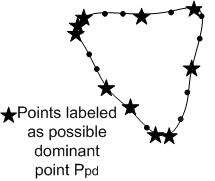
\includegraphics[scale=0.7]{images/ppd.jpg}
	\caption{Possible Dominante Points} An illustration of stroke points and the expected \textit{possible dominant points} $P_{pd}$.  
	%\label{fig:ppd}
	\label{fig:ppd999}	
\end{figure}

\subsection{Segmentation}
\label{seg}
In the segmentation stage, the input stroke is divided into a set of primitives. As shown in Figure \ref{fig:segblock} first an attempt is made to fit the stroke points into a curve or an ellipse using a minimum square error fitting algorithm \cite{ellipsefit}. The ellipse fitting step mainly helps to prevent the system from over segmenting the stroke into multiple lines or curves if the input stroke is an ellipse. If the stroke proved to be an ellipse arc then the segmentation process ends and the system proceeds to the next step. Otherwise, the stroke is passed to two further segmentation algorithms that divide the stroke to either lines or lines and curves. Hence we generate two different segmentations; the system chooses the segmentation with the minimum error. The following sections describe in details the ellipse detection algorithm and the two segmentation algorithms used to divide the stroke. 
 \begin{figure}
	\centering
		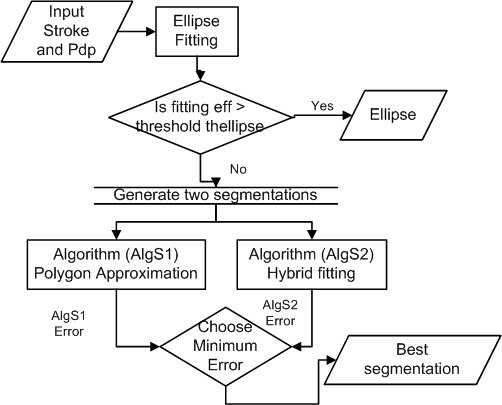
\includegraphics[scale=0.48]{images/flowchart.jpg}
	\caption{Segmentation process flow chart} Inputs to the segmentation proces are the input stroke and \textit{possible dominant points} $P_{pd}$. The output is either the stroke fitted as an ellipse or the best segmentation generated from the two segmentation algorithms.   
	\label{fig:segblock}
\end{figure}

 
\subsection{Ellipse fitting}
 
This process attempts to fit the stroke points into an ellipse arc; it starts by computing the center of the stroke bounding box. The bounding box center point is used as the first estimation of the center of the ellipse. The axis of the ellipse are estimated as the $width/2$ and $height/2$ of the stroke bounding box where $width$ and $height$ are the width and height of the bonding box. The least square fitting algorithm \cite{chernov} is used to minimize the fitting error of the ellipse Equation (\ref{eq:circleFit})  
\begin{equation}
E = \sum\limits_{i = 0}^N {\frac{{(x_i - x_0 )}}{{a^2 }}^2  + \frac{{(y_i - y_0 )}}{{b^2 }}^2  - 1} 
\label{eq:circleFit}
\end{equation}
where $N$ is number of points in the stroke, $a$ \& $b$ are the length of ellipse axes, $x_0$ \& $y_0$ are the coordinates of the center point and $x_i$ \& $y_i$ are the coordinates of point $i$ in the stroke. A list of new values for $x_0$ , $y_0$ ,$a$ and $b$ are generated randomly from the older values with small increments after each loop.  After few iterations, the final fit error of the estimated ellipse is reported. Another measure is used to compute the efficiency of the final estimated ellipse. The value of $eff$ in Equation \ref{eq:circleError} ensures that the drawn percentage of ellipse is considered. This eliminates fitting a line into very large ellipse but leaves small ellipses to be fitted as a partial or a full ellipse. 

 \begin{equation}
 eff= \begin{cases} 
\displaystyle \frac{P_{percent}}{E},&if P_{percent}< 0.5 \\ \medskip
\displaystyle  \frac{P_{percent}}{2\times E},&if P_{percent}\geq 0.5 \\
 
\end{cases},
\label{eq:circleError}
\end{equation}
 where $E$ is the error computed by Equation (\ref{eq:circleFit}), and 
\[
P_{percent}  = L_{stroke} /P_{ellipse}, 
%\label{eq:ErrorArea}
\]
 where $L_{stroke}$ total length of stroke and $P_{ellipse} $ is the perimeter of the estimated ellipse. If $eff$ has a value more than threshold $th_{Ellipse}$\footnote{By trial and error best threshold found was $th_{Ellipse}=0.2$} then the stroke is segmented as an ellipse otherwise the system proceeds to the next step. 

\subsection{Non ellipse fitting algorithm}
\label{subsubsec:Discreteparticleswarmalgorithm}
\begin{figure}
	\centering
 	 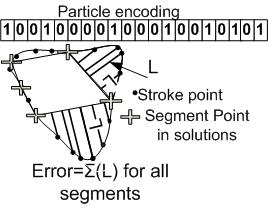
\includegraphics[scale=0.7]{images/pso1.jpg}			
	\caption{DPSO algorithm encoding} The swarm particle encoding where 1 represent the dominant points or segment points (i.e points are drawn as a big plus). Length L is the distance between a stroke point and the line connecting two successive segment points.  
	\label{fig:pso1}
\end{figure}
Two DPSO algorithms are used to generate different segmentations for each stroke the user draws. For each segmentation generated, an error is evaluated. The segmentation with the minimum error value is chosen as the best stroke segmentation (Figure \ref{fig:segblock}). The problem definition is the same in both algorithms but they differ in the method they use to compute fitness and error functions. 
\begin{description}
	\item[ Problem definition:] The input stroke $S$  with $N$ points can be represented by set $S = \left\{ {x_1 ,x_2  \ldots x_N }\right\}$ where $x_i$ is the location of the point $i$. The swarm algorithms consist of $M$ agents which are represented by the set $A = \left\{ {P_i \left| {i = 1,2 \cdots M} \right.} \right\}$ where $P_i$ is a single solution particle from the solution space. Each particle decodes the problem using a binary array with the same length $N$ as the input stroke.  

Therefore, the system represents each particle $P_i$ by $P_i = \left\{ {p_{ij} \left| {j = 1,2 \cdots N} \right.} \right\}$ where $p_{ij}$ has only two values a)1 ($p_{ij}=1$); means that this point ($j$) is a dominate point, or b) 0 ($p_{ij}=0$) means this point ($j$) is not a dominate point. Figure\ref{fig:pso1} shows a particle encoding in the DPSO system. 

	\item[Fitness function:] The fitness function and error calculation are different in each of the two \textit{DPSO} algorithms. 
	\end{description}
\subsubsection{\textit{Polygon Approximation Algorithm \textsl{(AlgS1)}}}
%\\
The approximation error is computed by the equation \ref{eq:ErrorSwarm1}. The graphical meaning of the error is shown in Figure\ref{fig:pso1}.
\begin{equation}
E=\sum\nolimits_{i = 0}^M e ( \widehat{x_ix_{i+1}},\overline{x_i x_{i+1}})
\label{eq:ErrorSwarm1}
\end{equation} where the arc $\widehat{x_ix_j}$ is defined as the consecutive set of points from point $x_i$ to point $x_{j}$ as in $x_i,x_{i+1} \cdots,x_j$. The line $\overline{x_i x_j}$ is defined as the straight line connecting point $x_i$ to point $x_j$ and $M$ is the number of dominant points in this solution as generated by the swarm algorithm. The error $e ( \widehat{x_ix_j},\overline{x_i x_j})$ is computed as the sum of squared perpendicular distance from every point along the arc $\widehat{x_ix_j}$ to the line $\overline{x_i x_j}$. The fitness is computed using the following equation %\ref{eq:fitnessSwarm1}

\begin{equation}
\max fitness(p_i ) = \left\{ {\begin{array}{*{30}l}
   {\displaystyle \frac{-E}{\varepsilon N}} & {ifE > \varepsilon }  \\ 
   
   { \frac {D}{\sum\limits_{j = 1}^N {p_{ij} } }} & {otherwise}  \\
\end{array}} \right.,
\label{eq:fitnessSwarm1}
\end{equation} where $N$ is the number of points in the stroke, $D$ is the number of points in the solution that were previously labeled as possible dominant points ($P_{pd}$), $E$ is the computed error and $\varepsilon$ is the error threshold. It should be noticed that when the error is larger than the threshold $\varepsilon$ the fitness is given a $-ve$ value to lower the fitness value of the solution. Otherwise, the system favors the least number of vertices.

 \subsubsection{\textit{Hybrid Fitting Algorithm \textsl{(AlgS2)}}}
The \textsl{(AlgS2)} algorithm has the same problem formulation as \textsl{(AlgS1)}. However, it has different fitness and error functions. An attempt is made to fit each segment into a line or circular arc. The errors of both circle and line fit estimations are computed for each segment $S_i=\widehat{x_ix_j}$. The approximation with the lowest error value is chosen as the final approximation of this segment $S_i$\cite{CruveDivisionSwarm}. The sum of the approximation errors of all segments is considered the total error of the particle. The total error of the particle is computed by equation %\ref{eq:errorSwarm2}
 \begin{equation}
E=\sum\nolimits_{i = 0}^{N_s} e(D_i) 
\label{eq:errorSwarm2}
\end{equation}where $N_s$ is the number of segments in the solution as generated by the swarm algorithm, $D_i$ is the minimum approximation error of curve and line approximations $min(d_c,d_l)$ where $d_c$ is the circle approximation error and $d_l$ is the line approximation error as computed by \cite{CruveDivisionSwarm}.  The fitness is computed by the equation %\ref{eq:fitnessSwarm2} 
\begin{equation}
\max fitness(P_i ) = \frac{1}{{E \times {N_s}^k }}
\label{eq:fitnessSwarm2}%$N_s$ is the number of segments and
\end{equation} where $E$ is the error and $k$ is a parameter tweaked to get minimum number of segments. The larger $k$ is, the higher the effect the number of segments will have. For our system, $k$ is selected to be 0.5 \cite{CruveDivisionSwarm}.

After each iteration of the swarm algorithm (\textsl{AlgS1} and \textsl{AlgS2}), each particle is refined using the following procedures: 
\begin{enumerate}
	\item For each particle $P_i$ each dominant point $P_{ij}$ is checked to find if it was labeled before as a \textit{possible dominant point} $P_{pd}$ (computed as in section \ref{Prepross}). If it was not labeled, the point $P_{ij}$ is moved to the nearest labeled point. This ensures that all of the points generated by the DPSO are possible dominant points $P_{pd}$. 
	\item The particles are tested to make sure that the distance between every two successive dominate point is larger than $min_D$, where $min_D$ is 5\% of the total length of the stroke.  Otherwise, two temperary particles are evaluated by removing either point from the current particle. After that, one of these points is removed based on the error caused by its removal.
	\item Each two successive segments are tested to determine if they can be merged into a single segment. If merging the two segments results in segmentation that has an error value less than or equal to the error before merging, the two segments are merged. This step ensures that the final segmentation of the system has minimum number of segments. 
	% the same or smaller the error
\end{enumerate}
%1) 2)  % If two points are nearer than $min_D$ then one of the points is removed. 
\subsection{Recognition}
\label{sec:Recognition}
After the user draws all strokes of the symbol, the set of un-recognized strokes is grouped together along with their segmentation as input to the feature extraction process. A composite set of features is used to generate a single feature vector. The following list describes each feature in details.
%\begin{description}
\subsubsection{Structural and geometrical Features (FS1)}
  They are features that define the structure of the geometrical symbol such as;   
 \begin{itemize}
	 \item \emph{Segments:} The number of segments in the symbol.
	 \item \emph{Strokes:} The number of strokes or partial strokes that created the symbols.  
		\item  \emph{Primitives:} The number of primitives in the symbol. This feature helps when identifying  symbols with mixed geometric primitives such as cylinders and callouts.  
		\item \emph{Curves:} The number of curves or ellipses in the symbol. 
		\item \emph{Lines:} The number of lines in the symbol. 
		\item \emph{Perpendicular}\emph{lines:} The number of perpendicular lines. 
		\item \emph{Parallel}\emph{lines:} The number of parallel lines. 
		\item \emph{Intersections:} The number of intersection between lines and curves. 
		\item \emph{T intersections:} The number of T intersections. 
		\item \emph{L intersections:} The number of L intersections. 
		\item \emph{X intersections:} The number of X intersections.	
 
\end{itemize}
\subsubsection{Rubine Features (FS2)}
  These features were introduced by Rubine \cite{gestureexample12} for single stroke gestures. Such as length of stroke, cosine of starting angle, smoothness of symbol and some features extracted from the bounding box of the symbol. 
  
\subsubsection{Statistical Features (FS3)} 
These features use moments and statistical properties such as;
\begin{itemize}
	\item \emph{Zernike moments:} The zernike moments are orthogonal moments which define the distribution of point in the input space. They are invariant to both reflection and rotation of the input shape \cite{ZerMomentOrthogonal}. %The zernike moment were used in \cite{HeloiseBeautification} t. 
\end{itemize}
\subsubsection{Composite Features (FS4)}
 These features are composites of different geometrical and statistical properties of the symbol. 
	\begin{itemize}
\item \emph{Size Ratio:} The ratio between width and height of the symbol.
	\item \emph{Ink density:} The density of points inside its bounding box\cite{GeometryAndDomain102}.   
 	\item \emph{Convex Hull Area:} The area of convex hull with respect to area of bounding box of symbol.
	\item \emph{Convex Hull Perimeter:} The perimeter of convex hull with respect to total length of symbol.
		\item \emph{Mean Centroidal radius:} The Mean of the centroidal radius is the distance from each point in the symbol to the center of gravity.
	\item \emph{Mean Time difference:} The mean of the time difference between each two successive points in the symbol. 
  \end{itemize}  
 
 After computing the features, the symbol is introduced to the classifier as a feature vector. The system uses Support Vector Machine (SVM) classifier with Linear kernel \cite{libsvm}. An OVO classifier structure (object versus object) is used to handle multi-class problem.% A validation algorithm is used to choose the Kernel variables parameters $c, \gamma$.

\section{Experimental}
\label{sec:Experiments} 
%Figure \ref{fig:symbolSet} shows a set of the shapes used in this data set. 
In our experiment we used three different datasets. The first dataset (Figure \ref{fig:HsSet}) was collected by Hse and Newton\cite{HeloiseBeautification} (Hs-DS). The data are drawn by 16 users each of them was asked to draw 13 shapes from 30 to 50 times. Figure \ref{fig:ELsymbolSet} and \ref{fig:LogicsymbolSet} shows the symbols we manually gathered from 7 different users in electrical (EL-DS) and logic design (LD-DS) domain respectively.  Table \ref{tab:datasets} shows a comparison between the three datasets used in our experiments. The datasets were divided into training and test sets. Five different splits for the training and test data are generated from each dataset. The results displayed are the average recognition accuracy of the five splits. The accuracy is computed as the number of correctly recognized samples divided by the total number of samples in the test. 
\begin{figure}
\centering 

\fbox{ \parbox{5cm}{% 
		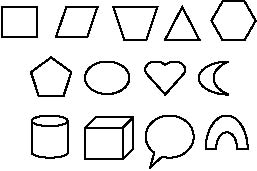
\includegraphics[scale=0.5]{images/symbolSet.PNG}	}}
		\caption{The Hs-DS Symbol Set} The dataset consist of simple presentation symbols.
		\label{fig:HsSet} 
\end{figure}

 \begin{figure}
			\subfigure[The Digital Design Symbols Dataset(LD-DS)]{\label{fig:LogicsymbolSet} 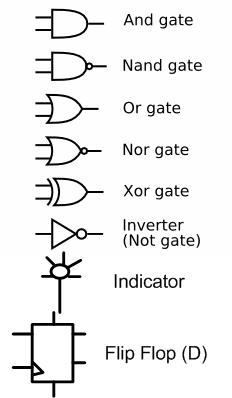
\includegraphics[scale=0.5]{images/logicSet.jpg}}
			\hfill
			\subfigure[The Electrical Symbols Dataset(EL-DS)]
			 {\label{fig:ELsymbolSet}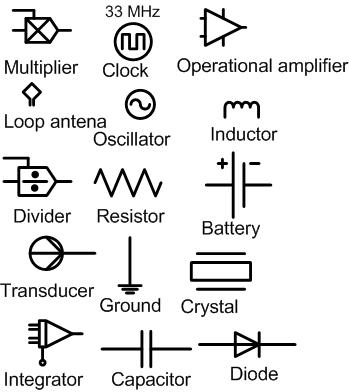
\includegraphics[scale=0.45]{images/EelectImage.jpg}}
 	
	\caption{The datasets that were manually collected}  a)  The (LD-DS) dataset consist of symbols that are visually similar (i.e. has low shape diversity). b) The (EL-DS) dataset consist of complex topological symbols. 
\end{figure}



\begin{table}
\begin{center}
\scalebox{0.8}{
 \begin{tabular}{|p{3cm}|p{1.5cm}|p{1.5cm}|p{1.5cm}|}
 \hline
 & Hs-DS &  EL-DS & LD-DS \\ \hline
No of samples  &  7791 & 2764 & 1859 \\ \hline
No of categories  & 13 & 15 & 8 \\ \hline
Avg. Samples per Category& 600 & 184 & 232 \\\hline 
No of users  & 16 & 7 & 7 \\  \hline
Balanced & Yes&No & No \\ \hline
Splits  & 5 random splits  & 5 random splits  & 5 random splits  \\ \hline
Examples & Figure \ref{fig:HsSet}  & Figure \ref{fig:ELsymbolSet}  & Figure \ref{fig:LogicsymbolSet}   \\ \hline
\end{tabular}
}
\caption[Datasets Comparisons]{Table compares between datasets used in experiments in terms of number of samples, number of samples per category, etc...} 
\label{tab:datasets}

\end{center}
\end{table}

A set of tests were performed on the system to enhance non-ellipse fitting algorithms. The effect of the number of particles, the error thresholds and various other parameters were investigated. The results of these tests are shown in Figures \ref{fig:swarmtesting} and   \ref{fig:swarmtesting2}. Figure \ref{fig:swarmtesting} shows that as the number of swarm iterations increase the error value decrease (error of the segmentation algorithm). The final number of particles and maximum swarm iterations used in the system was based on a tradeoff between error achieved versus the computation time. The effect of other algorithm parameters such as $c_1$, $\omega$ (mentioned in Section\ref{sec:ParticleSwarmAlgorithm}) is tested using similar tests (Figure  \ref{fig:swarmtesting2},\ref{fig:swarmwtest}).%, $c_2$ 
    
 \begin{figure}
	\centering		
	 	\subfigure[Segmentation Error Vs. Swarm Iterations]{	\label{fig:swarmtesting} 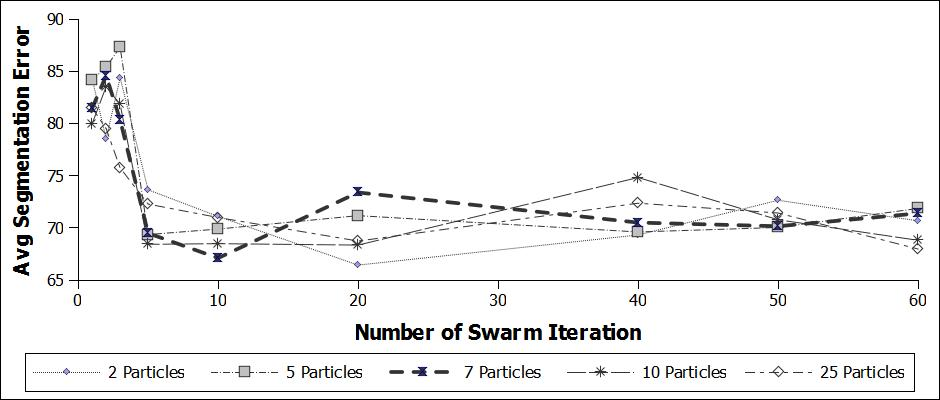
\includegraphics[scale=0.3]{images/swarmIterationVsParticles.jpg}}
  
		\subfigure[Segmentation Error Vs. $c_1$]{	\label{fig:swarmtesting2}  \includegraphics[scale=0.3]{images/C1Swarm.jpg}} %swarmParamterC.jpg
		
				\subfigure[Segmentation Error Vs. $\omega$]{\label{fig:swarmwtest}  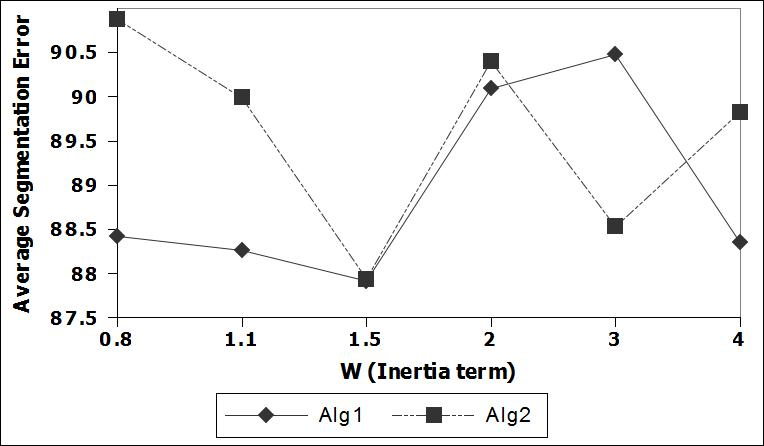
\includegraphics[scale=0.3]{images/wSwarm.jpg}} %swarmParamterC.jpg
		
	
		
	 	\caption{Segmentation Error Vs. PSO parameters.}a) The error decrease as the number of swarm iteration increase until it reach a saturation.   b) The behavior of segmentation error versus $c_1$. c) The behavior of segmentation error versus  $\omega$
	 
 	
\end{figure} 
\subsection{Algorithms comparisons}
\label{sec:AlgExp}
We performed several experiments to evaluate the presented recognition system. Firstly, we tested recognition accuracy of shapes in the data set with both algorithms (\textsl{AlgS1} and \textsl{AlgS2}). We also implemented the segmentation algorithm described in \cite{earlyprocess} (\textsl{Alg3}) to compare it with our swarm algorithms. Figure \ref{fig:test1} and \ref{fig:testLD} show the accuracy achieved by each algorithm. The two swarm algorithms were tested with and without the ellipse fitting module. Combining the ellipse detection module improves the performance in certain datasets. The result shows that (\textsl{AlgS2}) gives better performance than Alg3 and AlgS1 in all datasets.  The results also shows that combining (\textsl{AlgS1} and \textsl{AlgS2} using minimum error) outperforms AlgS2 in Hs-Ds only. This behavior is explained by noticing that features are computed based on the chosen segmentation. This means that different segmentation for a symbol generates a different set of features used for recognition. This behavior affects Ls-Ds and EL-Ds more than Hs-Ds due to the higher topological and structure nature of the symbols in both datasets than of Hs-Ds. 

 \begin{figure} 
	\centering		
	\subfigure[Algorithm comparison on HS-DS]{\label{fig:test1} 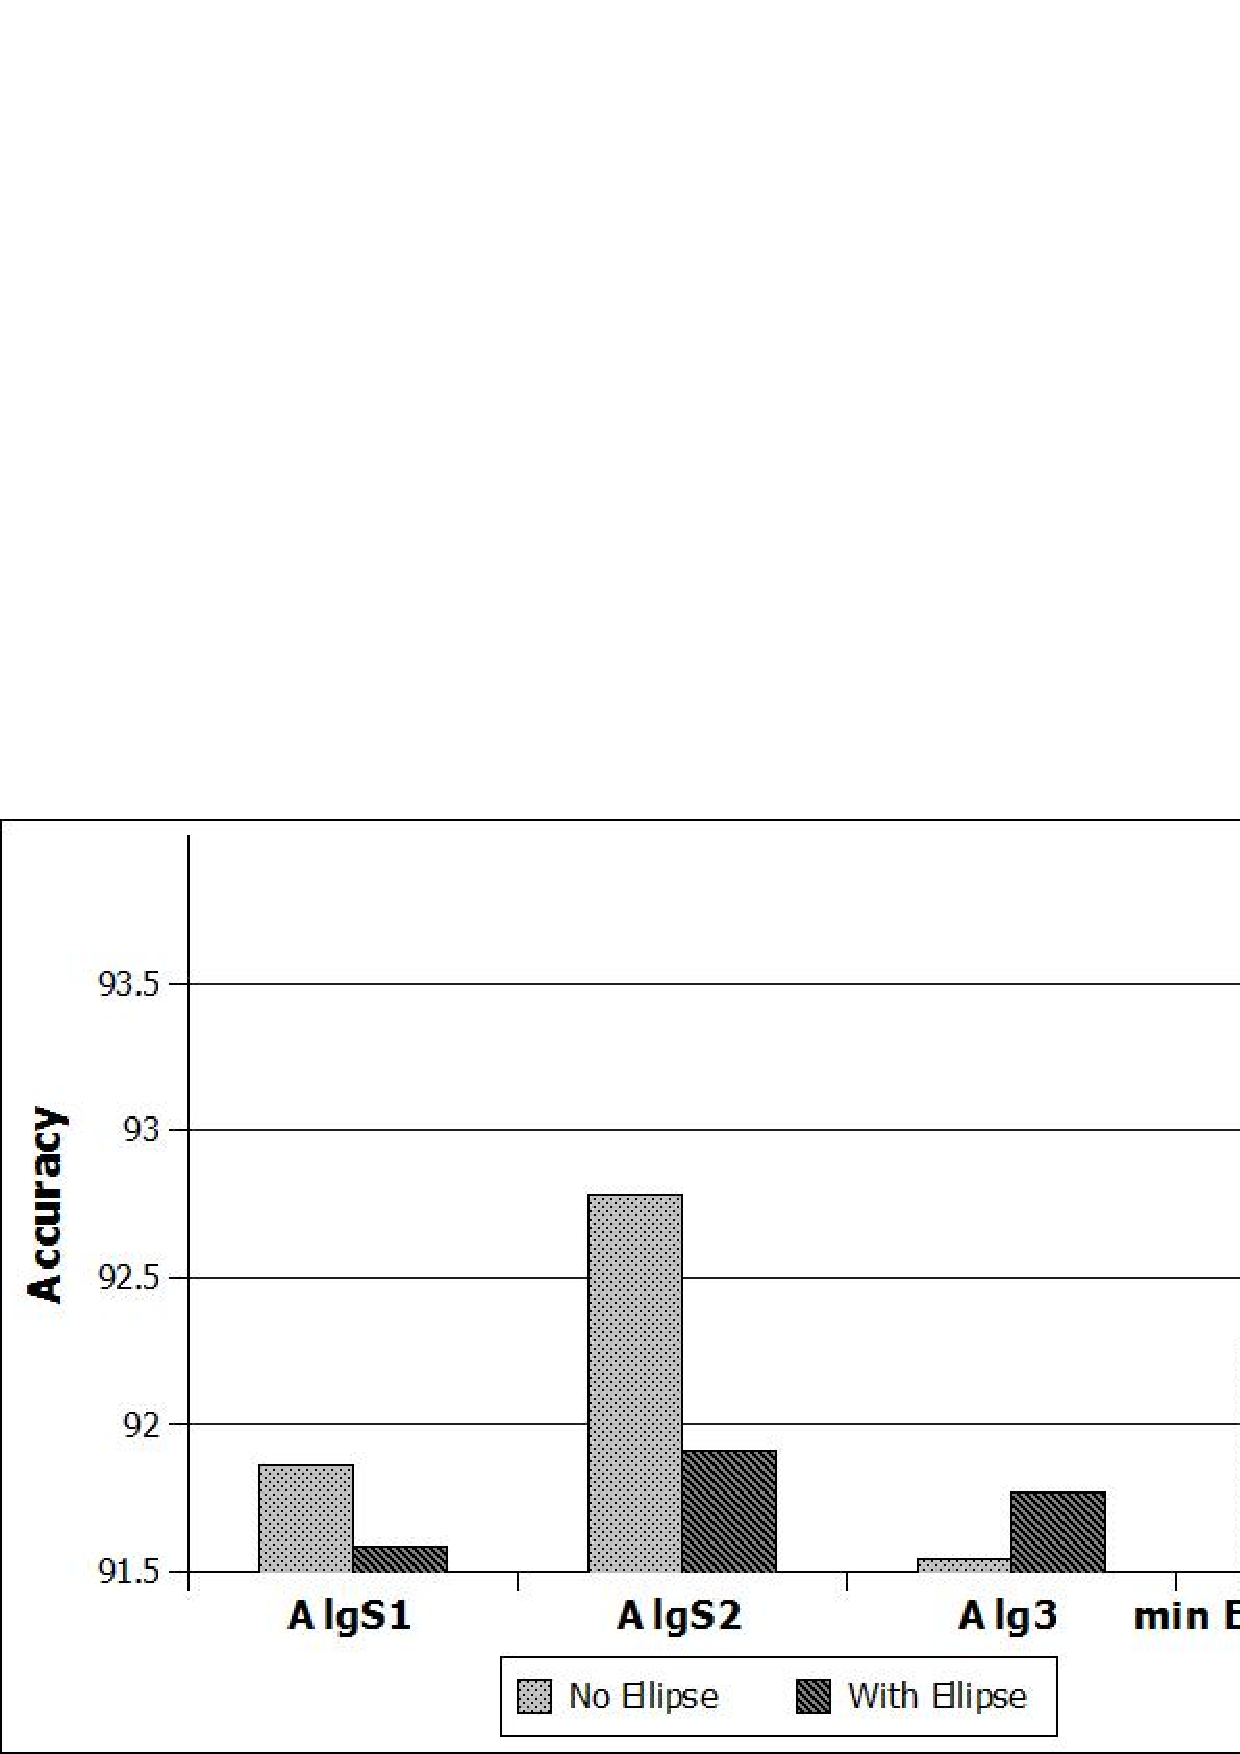
\includegraphics[scale=0.4]{images/testAlg.jpg}}
 		\subfigure[Algorithm comparison on LD-DS]{ 	 	\label{fig:testLD} 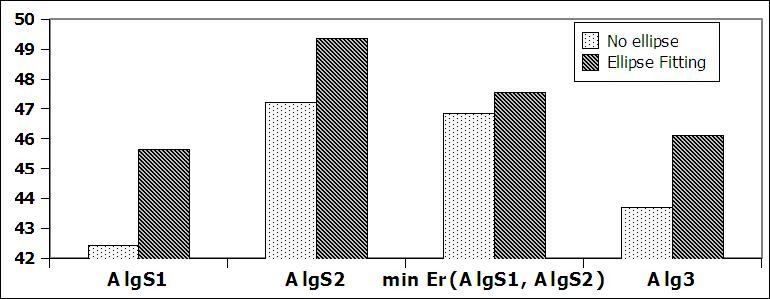
\includegraphics[scale=0.4]{images/LDAlg.jpg}}
 		\subfigure[Algorithm comparison on EL-DS]{	 	\label{fig:testEL}  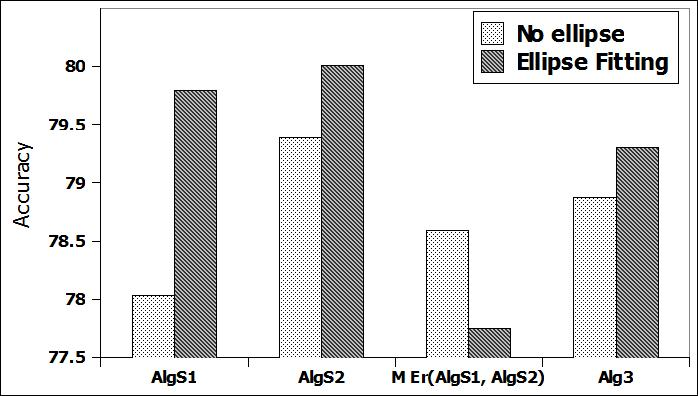
\includegraphics[scale=0.4]{images/AlgEL.jpg}}
	 	\caption{ The recognition rate of different algorithms. }
 \end{figure} 


\subsection{Shape Complexity Analysis}
\label{sec:ShapeComplexityExperiments}
The second experiment we implemented was to investigate the effect of symbol complexity and its type on the recognition rate. Figure \ref{fig:test2} and \ref{fig:LDtest2} show the achieved accuracy of each symbol by our algorithms compared to (\textsl{Alg3}) \cite{earlyprocess}. It is clearly noted that symbols that have only line segments achieve higher accuracy rate than other symbols (such as square, parallegram). The results also indicate that algorithm \textsl{AlgS1} achieves better performance than algorithm \textsl{AlgS2} in the symbols that consists only of lines. This is understandable because algorithm \textsl{AlgS1} divides strokes into line segments only but \textsl{AlgS2} is able to divide strokes into lines and curves based on the minimum error of the segment itself. Figure \ref{fig:LDtest2} shows that in logic design (LD-DS) \textsl{AlgS2} achieved better performance than \textsl{Alg3} and  \textsl{AlgS1}.  This proves that for complex shapes that are combination of lines and arcs are \textsl{AlgS2} achieves better segmentation. Algorithm \textsl{Alg3} gives good performance as long as the symbols consist of combination of lines and curves, if the stroke consists of curve or lines only the algorithm may lead to wrong segmentation result. This is because the system divides the stroke first into line segments then tries to decide whether each segment can be represented better as a curve. However, in \textsl{AlgS2} the curve segments are tested while choosing the best segmentation. Combining both algorithm \textsl{AlgS1} and \textsl{AlgS2} improved the recognition rate of all symbols. The penalty for this improved performance is the computational time required to run both swarm algorithms. Table \ref{tab:ConfusionMatrix} shows the confusion matrix for the (HS-DS) symbols. The table shows that an error occurs mostly between two sets of symbols: moon with triangles and trapezoid with triangles. This observation is understandable as the symbols are visually similar but the system must be able to differentiate between them. This leads us to the next experiment to choose the best set of feature to recognize symbols. 
\begin{figure*} 
	\centering 
		\subfigure[Symbols Comparison on HS-DS]{\label{fig:test2}
		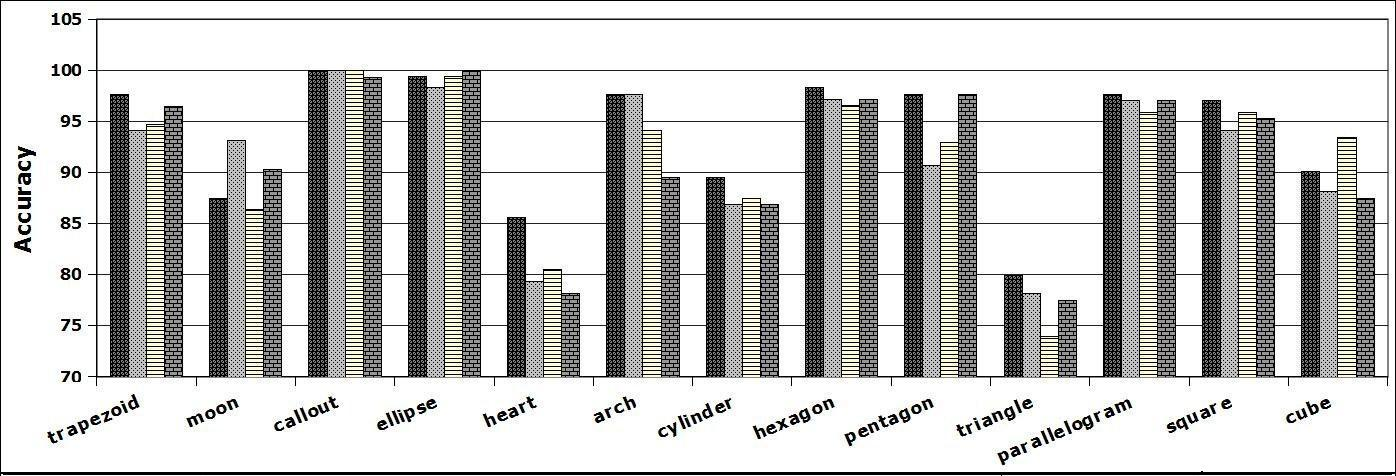
\includegraphics[scale=0.35]{images/testsym.jpg}}
\subfigure[Symbols Comparison on LD-DS symbols]{\label{fig:LDtest2}
		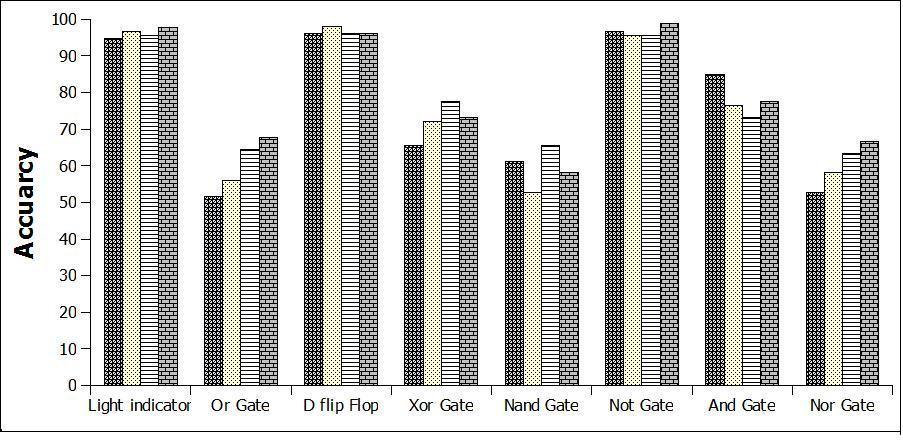
\includegraphics[scale=0.5]{images/DLSymbols.jpg}}
		\subfigure{ 
		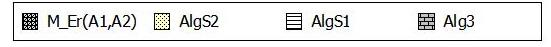
\includegraphics[scale=0.5]{images/captionSymbols.jpg}}
	%\caption{}.  %The graph shows the recognition rate of each symbol using different algorithms. 
	\caption {Symbol Comparison} The accuracy of achieved by each algorithm in each symbol. a) Low accuracy level appears in triangle, heart, and moon symbols. b) Low accuracy level appears only in symbols that are visually confusing (i.e Nor, OR, Nand gates). 
\end{figure*}  
\begin{table*}
	\centering
	%\small
%	\scalebox{0.7}{
		%	\begin{tabular}{|c|c|c|c|c|c|c|c|c|c|c|c|c|c|}\hline 
 %%%%%%%%%%%%%%%%%%%%%%%%%%%%%%%%%%%%%%%%%%%%%%%%%%%%%%%%%%%%%%%%%%%%%%
%%                                                                  %%
%%  This is a LaTeX2e table fragment exported from Gnumeric.        %%
%%                                                                  %%
%%%%%%%%%%%%%%%%%%%%%%%%%%%%%%%%%%%%%%%%%%%%%%%%%%%%%%%%%%%%%%%%%%%%%%
	\scalebox{0.5}{  % this was taken from algfeat from  Results_17-04-2009_07-13
			\begin{tabular}{|c|c|c|c|c|c|c|c|c|c|c|c|c|c|}\hline 
 Categories 	&ellipse	&heart	&trapezoid	&pentagon	&arch	&hexagon	&square	&triangle	&cube	&cylinder	&parallelogram	&moon	&callout\\ \hline 
ellipse	&150	&20	&0	&0	&0	&5	&1	&0	&0	&0	&0	&1	&0\\  \hline 
heart	&2	&130	&0	&1	&10	&1	&1	&0	&0	&0	&1	&4	&0\\  \hline 
trapezoid	&0	&1	&147	&5	&1	&0	&1	&3	&2	&0	&37	&0	&0\\  \hline 
pentagon	&0	&0	&1	&139	&0	&7	&0	&0	&0	&0	&1	&0	&0\\   \hline 
arch	&0	&0	&1	&1	&125	&0	&4	&0	&3	&0	&0	&15	&1\\   \hline 
hexagon	&0	&0	&0	&2	&0	&135	&0	&0	&0	&0	&0	&0	&0\\  \hline 
square	&0	&0	&0	&0	&0	&0	&138	&0	&0	&0	&0	&1	&0\\   \hline 
triangle	&0	&0	&1	&2	&5	&0	&1	&148	&0	&0	&4	&7	&0\\  \hline 
cube	&0	&0	&0	&1	&0	&0	&0	&0	&146	&5	&0	&0	&0\\   \hline 
cylinder	&0	&0	&0	&1	&0	&1	&0	&0	&0	&147	&0	&0	&0\\  \hline 
parallelogram	&0	&0	&0	&0	&0	&0	&2	&0	&2	&0	&107	&0	&0\\  \hline 
moon	&0	&1	&0	&0	&10	&2	&3	&0	&0	&0	&0	&125	&5\\   \hline 
callout	&0	&0	&0	&0	&0	&0	&0	&0	&0	&0	&0	&0	&145\\  \hline 
 		\end{tabular}
%		\begin{tabular}{|c|c|c|c|c|c|c|c|c|c|c|c|c|c|}\hline 
%  Categories 	&ellipse	&heart	&trapezoid	&pentagon	&arch	&hexagon	&square	&triangle	&cube	&cylinder	&parallelogram	&moon	&callout\\ \hline
%ellipse	&143	&4	&0	&0	&0	&0	&0	&2	&0	&0	&0	&0	&0\\ \hline
%heart	&7	&125	&0	&0	&0	&0	&0	&0	&0	&0	&0	&10	&0\\ \hline
%trapezoid	&0	&0	&147	&0	&2	&0	&2	&8	&0	&0	&2	&0	&0\\ \hline
%pentagon	&0	&0	&0	&138	&0	&1	&0	&0	&0	&0	&0	&2	&0\\ \hline
%arch	&0	&4	&0	&0	&138	&0	&0	&0	&0	&0	&0	&11	&0\\ \hline
%hexagon	&0	&1	&0	&5	&0	&152	&0	&0	&0	&0	&0	&0	&0\\ \hline
%square	&0	&0	&0	&0	&0	&0	&132	&0	&0	&0	&0	&0	&0\\ \hline
%triangle	&0	&0	&2	&0	&0	&0	&1	&136	&0	&0	&0	&1	&0\\ \hline
%cube	&0	&0	&0	&0	&0	&0	&1	&0	&142	&29	&14	&0	&0\\ \hline
%cylinder	&0	&0	&0	&0	&0	&0	&10	&0	&10	&120	&0	&0	&0\\ \hline
%parallelogram	&0	&0	&1	&0	&0	&0	&1	&2	&0	&0	&134	&0	&0\\ \hline
%moon	&2	&1	&0	&0	&3	&0	&3	&2	&0	&0	&0	&117	&0\\ \hline
%callout	&1	&15	&0	&7	&7	&1	&0	&1	&0	&1	&0	&9	&150\\ \hline
%		\end{tabular}
			}
			
 		%\end{tabular}
 	%}
	\caption{Confusion Matrix of Hs-DS}
	\label{tab:ConfusionMatrix}
	%\end{minipage}
\end{table*}
 \subsection{Features Analysis}
\label{sec:featexp}
%Results show that (\textbf{FS2}) Rubine features \cite{gestureexample12} gives the worst results when used alone without any other features.
Different feature sets are tested to determine the best features that can be used in sketch and symbol recognition. Figure\ref{fig:testFeaturesAll} shows the result of using different feature sets (from the basic four sets \textbf{FS1,FS2,FS3,FS4} in Section \ref{sec:Recognition}). Results show that geometerical features (\textbf{FS1}) and Rubine features (\textbf{FS2}) \cite{gestureexample12} give the low results when used alone without any other features. This is because they are mainly computed for single stroke gestures and fare badly in multi-stroke symbols \cite{compareFeaturSVM}. Features \textbf{(FS4)} give good results and it is further improved by adding geometerical structural features \textbf{(FS1)}.

 \begin{figure*}
	\centering
	\subfigure[Feature Comparison on Hs-DS]{	\label{fig:testFeaturesAll} 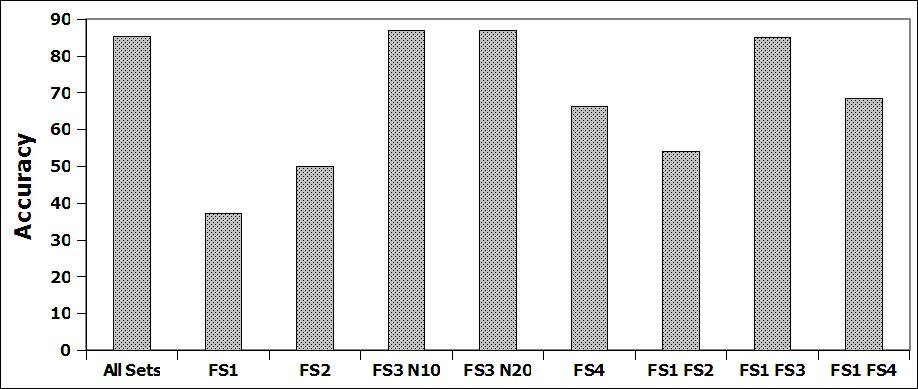
\includegraphics[scale=0.5]{images/featuresdifference.jpg}}
	\subfigure[Feature Comparison on EL-DS]{	\label{fig:ELtestFeaturesAll}	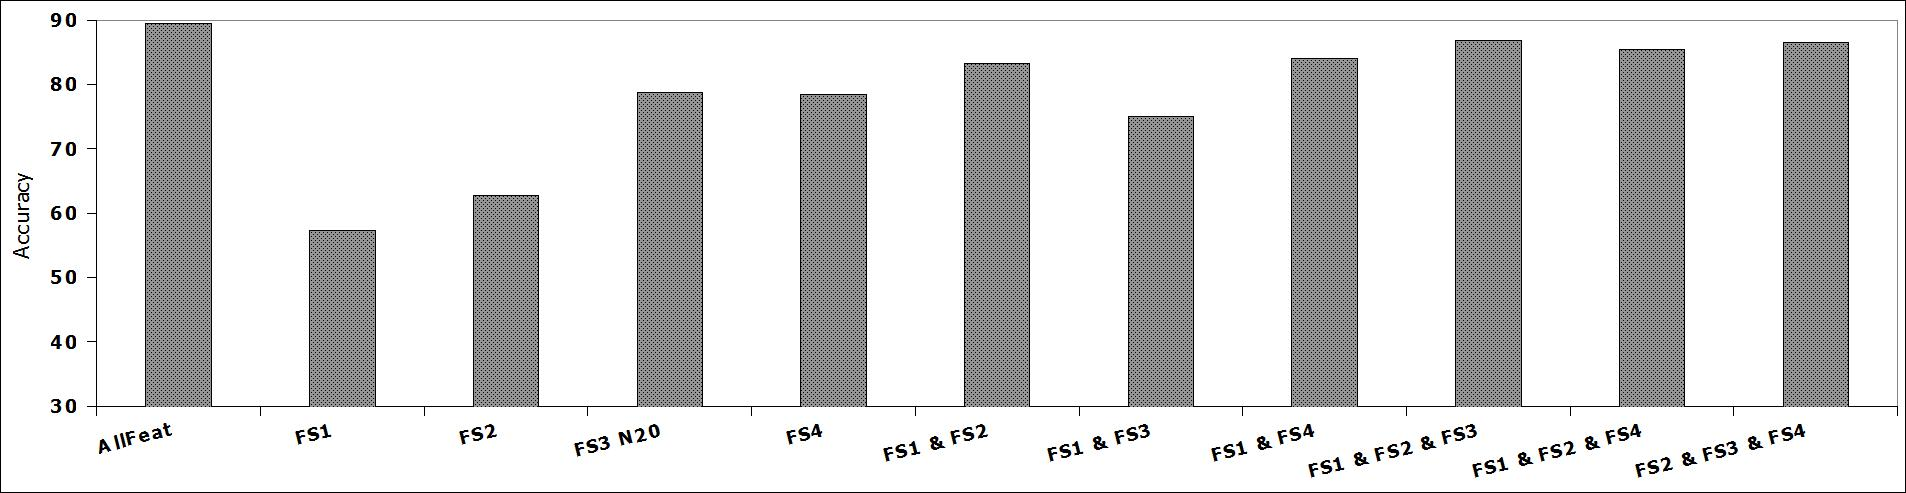
\includegraphics[scale=0.34]{images/FeatEl.jpg}}
	\caption{Different Features} The effect of different feature set on accuracy.  FS4 and FS3 give good results in a) Hs-DS and b) EL-Ds. The results are improved by combining FS1 with FS2 and FS1 with FS4.    %The graph shows the recognition rate of each symbol using different algorithms. 
\end{figure*}  

 We could not test the result of the segmentation algorithm alone due to the fact that the correct segmentation is highly qualitative. It is only based on what the user intends to draw while sketching the symbol. 
 
 The main features affected by the segmentation stage are the geometric features computed in \textbf{FS1}. Hence those are the features we used to estimate the efficiency of the segmentation algorithm. The recognition accuracy using only the geometrical features is reported in Figure \ref{fig:testFeatonly}. The figure shows that \textsl{AlgS2} achieve better results.  
\begin{figure*} 
	\centering
		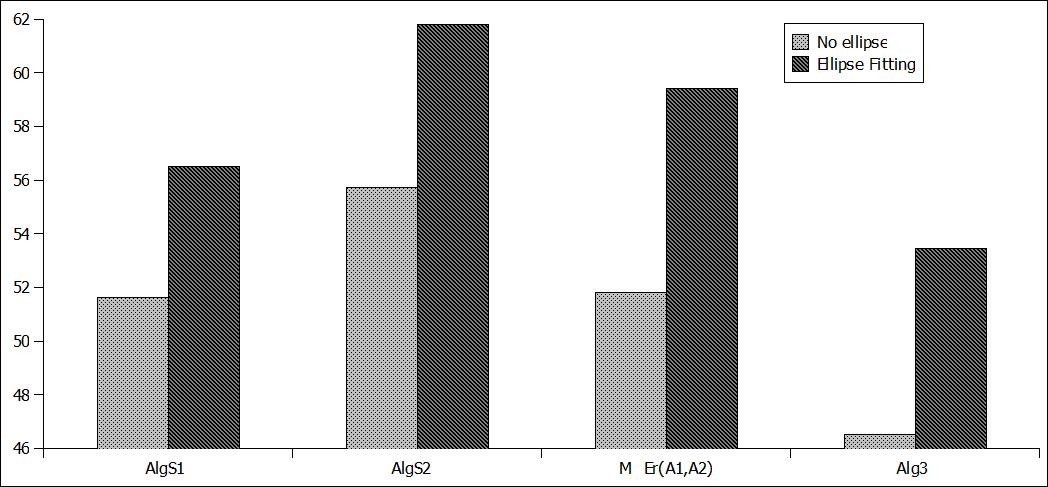
\includegraphics[scale=0.45]{images/OnlyF1EL.jpg}
	\caption{The effect of segmentation on accuracy} The experiment is implemented on Hs-Ds using only FS1.  %The effect of symbol complexity.  %The graph shows the recognition rate of each symbol using different algorithms. 
	\label{fig:testFeatonly}
\end{figure*}  

\begin{figure}[]
	\centering
				\subfigure[User strokes] {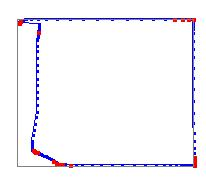
\includegraphics[scale=0.7]{images/strokebefore.jpg}}
		 	\subfigure[Segmented strokes] {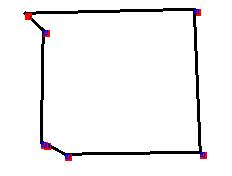
\includegraphics[scale=0.7]{images/strokeafter.jpg}}
		 		\subfigure[Multiple symbols] {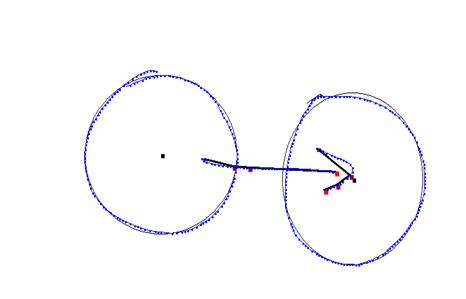
\includegraphics[scale=0.7]{images/results3.jpg}}
		
	\caption{Segmentation outputs} The output segmentation of different input strokes. a) Sample of single input stroke b) The single stroke after segmentation. c) An example of multiple strokes and their segmentation.   identified.
	\label{fig:SampleSeg}
\end{figure}

\section{Conclusion and Future Work}
\label{ConclusionandFutureWork}

This paper presented a new approach to sketch recognition using DPSO. The system uses multiple preliminary information, i.e., speed and curvature information, as input to the \textit{DPSO}. Results show that the \textit{DPSO} in general generates an optimized stroke segmentation which improves the final recognition rate.  The final recognition is based on both global shape and hierarchical stroke properties. Adding stroke and segment geometrical features improved the final recognition. Global shape and moment properties were used to prevent the need to use graph matching which is computationally expensive \cite{SketchRead2007}. The experiments evaluated two \textit{DPSO} different segmentation algorithms (AlgS1 and AlgS2) on three different datasets (Hs-Ds, EL-Ds and LD-Ds). Results show that AlgS2 achieves better segmentation and final accuracy than Alg3 \cite{earlyprocess} on the datasets used. The results proved that the system is easily expandable to more and more symbols as it does not depend on low level primitive recognizers but on high level symbol and geometrical features.  The system achieved an average overall improvement of more than 2\% over Alg3 in all datasets.  

  The tradeoff between accuracy achieved and time complexity can be further investigated to achieve better results. Currently, the system processes one symbol at a time, an enhancement would be to allow users to draw more than one symbol at a time and incorporate a method for separating symbols. Thus, possible extension of this research is to complete the clustering algorithm for fully automated sketch recognition. Another area of enhancements is the features extraction methods. Introducing more spatial and geometrical features is believed to improve classifications. Features that represent the appearance of the symbols are likely to improve the recognition of symbols that have similar geometrical structure (i.e. Nor and OR gate in logic symbols).  
 \bibliographystyle{elsarticle-harv} 
%\bibliographystyle{IEEEbib}
\bibliography{../../neededfiles/Bibliographies/Mybibliography}
\end{document}
